\documentclass[12pt]{book}


\usepackage{tabularx}
\usepackage[table]{xcolor}
\usepackage{multirow}

\usepackage{epigraph}

\usepackage[siunitx, RPvoltages]{circuitikz}
\usepackage{ifthen}
\usepackage{tikz}
\usepackage{pgf}
\usepackage{pgffor}
\usepgfmodule{plot}
\usepgfmodule{shapes}
\usepgfmodule{plot}
\usetikzlibrary{decorations.pathmorphing}
\usetikzlibrary{arrows}
\usetikzlibrary{shapes}
\usetikzlibrary{snakes}
\usepackage{siunitx} % for battery
\usepackage{steinmetz} % for phasor angle
\usepackage[margin=1.1in,footskip=.25in]{geometry}

\usepackage[most]{tcolorbox}
\usepackage{color}

\definecolor{codepurple}{rgb}{0.58,0.8,0.82}
\definecolor{backcolour}{rgb}{0.95,0.95,0.92}

\tcbset{
    frame code={}
    center title,
    left=10pt,
    right=10pt,
    top=10pt,
    bottom=10pt,
    colback=gray!5,
    colframe=gray,
    width=\dimexpr\textwidth\relax,
    enlarge left by=0mm,
    boxsep=5pt,
    arc=0pt,outer arc=0pt,
}

\usepackage{amsmath, amssymb}
\usepackage{mathtools}

\renewcommand{\baselinestretch}{1.3} 







\newcommand{\Gitter}[4]{
    \draw[very thin,color=gray] (#1,#3) grid (#2,#4);
}
\newcommand{\Koordinatenkreuz}[6]{
    \draw[->, >=latex, color=green!50!black] (#1,0) -- (#2,0) node[right] {#5};
    \draw[->, >=latex, color=green!50!black] (0,#3) -- (0,#4) node[left] {#6};
}
\newcommand{\KoordinatenkreuzOhneLabelsVerschobenKeinPfeil}[5]{
    \draw[-] (#1,0) -- (#2,0);
    \draw[-] (#5,#3) -- (#5,#4);

}
\newcommand{\ZeigerdiagrammText}[4]{
\begin{tikzpicture}[scale=.72, samples=100, >=latex,line width = 1pt]

    \def\Alpha{#1}
    \def\Phase{#2}
    \def\AmplitudeSpannung{#3}
    \def\AmplitudeStrom{#4}
    \def\SpannungsWert{{\AmplitudeSpannung*sin(\Alpha)}}
    \def\StromWert{{\AmplitudeStrom*sin(\Alpha+\Phase)}}
    %%%%%%%%%%%%%%%%%%%%%%%%%%%%%%%%%%%%%%%%%%%%%%%%%%%%%%%%%%
    \def\FarbeSpannung{blue!90!white}
    \def\FarbeStrom{red!90!white}
    \def\FarbeWinkelZeichnung{green}
    %%%%%%%%%%%%%%%%%%%%%%%%%%%%%%%%%%%%%%%%%%%%%%%%%%%%%%%%%%
    \def\Beta{\Alpha+\Phase}
    \def\AlphaRad{\Alpha*3.141592654/180}
    \def\PhaseRad{\Phase*3.141592654/180}
    %%%%%%%%%%%%%%%%%%%%%%%%%%%%%%%%%%%%%%%%%%%%%%%%%%%%%%%%%%
    \Gitter{-.1}{7.1}{-3.1}{3.1}
    \Koordinatenkreuz{-.2}{7.3}{-3.2}{3.3}{$\omega t$}{$V(t)$}
    \draw (1.570795,0) node[below]{$\frac{\pi}{2}$};
    \draw (3.14159,0) node[below]{${\pi}$};
    \draw (4.71238898,0) node[below]{$\frac{3\pi}{2}$};
    \draw (6.283185307,0) node[below]{${2\pi}$};
    \draw (-4,0) circle (3cm);
    \KoordinatenkreuzOhneLabelsVerschobenKeinPfeil{-7.2}{-.8}{-3.6}{3.6}{-4}
    %%%%%%%%%%%%%%%%%%%%%%%%%%%%%%%%%%%%%%%%%%%%%%%%%%%%%%%%%%

    % voltage
    \draw[color=\FarbeSpannung, very thick] plot[id=voltage, domain=0:7] function{\AmplitudeSpannung*sin(x)} ;
    % voltage circle
    \draw[color=\FarbeSpannung, loosely dashed] (-4,0) circle (\AmplitudeSpannung cm);
    % angle
    \draw[color=\FarbeWinkelZeichnung!50!black, thick] (\AlphaRad, \SpannungsWert)--(\AlphaRad,\StromWert) node[below=18pt] {$\alpha$};
    % angle in the circle
    \filldraw[fill=\FarbeWinkelZeichnung!20,draw=\FarbeWinkelZeichnung!50!black] (-4,0) -- (-3,0) arc (0:\Alpha:1) -- cycle node[right] {$\alpha$};
    % voltage pointer
    \draw[<-,color=\FarbeSpannung, very thick] (\Alpha:\AmplitudeSpannung)++(-4,0) --(-4,0);
    \draw[color=\FarbeSpannung,  dashed] (\Alpha:\AmplitudeSpannung)++(-4,0) -- (\AlphaRad,\SpannungsWert);
    % current
    \draw[color=\FarbeStrom, very thick] plot[id=current, domain=0:7] function{\AmplitudeStrom*sin(x+\PhaseRad)};		
    % current circle
    \draw[color=\FarbeStrom, loosely dashed]    (-4,0) circle (\AmplitudeStrom cm);
    % current pointer
    \draw[<-,color=\FarbeStrom, very thick] (\Beta:\AmplitudeStrom)++(-4,0) --(-4,0);
    \draw[color=\FarbeStrom,  dashed](\Beta:\AmplitudeStrom)++(-4,0) -- (\AlphaRad,\StromWert);
    % phase difference
    \ifthenelse{\Phase<0}{
        \draw[snake=brace] (pi/2 ,3.3)--(pi/2-\PhaseRad ,3.3) node[above=7pt, left=10pt] {$\phi$};
    }
    {
        \draw[snake=brace] (pi/2-\PhaseRad ,3.3)--(pi/2 ,3.3) node[above=7pt, left=10pt] {$\phi$};
    }
    % angular velocity \omega
    \draw[->, xshift=-4cm]  (120:2.4cm) arc (120:170:2) node[below] {$\omega$};
\end{tikzpicture}
}


\renewcommand\epigraphflush{flushright}
\renewcommand\epigraphsize{\normalsize}
\setlength\epigraphwidth{0.7\textwidth}

\definecolor{titlepagecolor}{cmyk}{1,.60,0,.40}

\DeclareFixedFont{\titlefont}{T1}{ppl}{b}{it}{0.5in}


\newcommand\titlepagedecoration{%
\begin{tikzpicture}[remember picture,overlay,shorten >= -10pt]

\coordinate (aux1) at ([yshift=-15pt]current page.north east);
\coordinate (aux2) at ([yshift=-410pt]current page.north east);
\coordinate (aux3) at ([xshift=-4.5cm]current page.north east);
\coordinate (aux4) at ([yshift=-150pt]current page.north east);

\begin{scope}[titlepagecolor!40,line width=12pt,rounded corners=12pt]
\draw
  (aux1) -- coordinate (a)
  ++(225:5) --
  ++(-45:5.1) coordinate (b);
\draw[shorten <= -10pt]
  (aux3) --
  (a) --
  (aux1);
\draw[opacity=0.6,titlepagecolor,shorten <= -10pt]
  (b) --
  ++(225:2.2) --
  ++(-45:2.2);
\end{scope}
\draw[titlepagecolor,line width=8pt,rounded corners=8pt,shorten <= -10pt]
  (aux4) --
  ++(225:0.8) --
  ++(-45:0.8);
\begin{scope}[titlepagecolor!70,line width=6pt,rounded corners=8pt]
\draw[shorten <= -10pt]
  (aux2) --
  ++(225:3) coordinate[pos=0.45] (c) --
  ++(-45:3.1);
\draw
  (aux2) --
  (c) --
  ++(135:2.5) --
  ++(45:2.5) --
  ++(-45:2.5) coordinate[pos=0.3] (d);   
\draw 
  (d) -- +(45:1);
\end{scope}
\end{tikzpicture}%
}

\usepackage{xepersian}
\settextfont{Vazir}

\begin{document}

%\title{مدار الکتریکی}

%\maketitle

\begin{titlepage}
%\noindent
\titlefont 
\begin{tikzpicture}
\begin{scope}
\node[scale=4] (b) at (2,-2) {الکتریکی مدار};
\end{scope}
\end{tikzpicture}


\null\vfill
\vspace*{1cm}
\noindent
\hfill

\titlepagedecoration
\end{titlepage}

\tableofcontents

\chapter{مقاومت تونن و جریان نورتن}

\section{نحوه ی تعیین مقاومت تونن و جریان نورتن}

\begin{enumerate}
	\item همه ی منابع ولتاژ و جریان مستقل را خاموش می کنیم ، سپس مقاومت معادل را از  دو سر ترمینال مورد نظر به دست می آوریم .
	\item برای به دست آوردن 
	$V_{th}$
	ترمینال مورد نظر را باز می کنیم و ولتاژ مدار باز را به دست می آوریم 
	$$
	V_{OC} = V_{open \:\: circuit} = V_{th}
	$$
	\item برای به دست آوردن 
	$I_{N}$
     یا جریان مدار باز ، ترمینال  
	مورد نظر را اتصال کوتاه می کنیم .
	$$
	I_{SC} = I_{short \:\: circuit} = I_{N}
	$$
\end{enumerate}



\begin{circuitikz}[american]
 \draw (0,-1) to[V=$V_{th}$] (0,1);
 \draw (0,1) to[R=$R_{th}$] (3,1) node[right] {$A$};
 \draw (0,-1) -- (3,-1) node[right] {$B$};
 \begin{scope}[xshift=8cm]
 \draw (0,-1) to[isource, l=$I_{N}$] (0,1);
 \draw (2,-1) to[R=$R_{th}$] (2,1) ;
 \draw (0,1) -- (3,1) node[right] {$A$};
 \draw (0,-1) -- (3,-1) node[right] {$B$};
 \end{scope}
\end{circuitikz}

$$
I_{N} = \frac{V_{th}}{R_{th}}
$$


\newpage

\subsubsection{مثال}

در مدار شکل زیر مقاومت تونن و جریان نورتن را به دست آورید ؟


\begin{circuitikz}[american]
 \draw (0,-1) to[V=\SI{18}{v}] (0,1);
 \draw (0,1) to[R=$3$] (3,1) -- (6,1) node[right] {$A$};
 \draw (0,-1) -- (6,-1) node[right] {$B$};
 \draw (3,-1) to[R=$6$] (3,1);
\end{circuitikz}


برای به دست آوردن مقاومت تونن منابع ولتاژ را خاموش می کنیم ، یعنی اتصال کوتاه می کنیم


\begin{circuitikz}[american]
 \draw (0,-1) -- (0,1);
 \draw (0,1) to[R=$3$] (3,1) -- (6,1) node[right] {$A$};
 \draw (0,-1) -- (6,-1) node[right] {$B$};
 \draw (3,-1) to[R=$6$] (3,1);
\end{circuitikz}

$$
R_{th} = \frac{3 \times 6}{3 + 6} = \frac{18}{9} = 2 \:\: \Omega
$$

برای به دست آوردن 
$I_{N}$
، A و  B
را اتصال کوتاه می کنیم .

\begin{circuitikz}[american]
 \draw (0,-1) to[V=\SI{18}{v}] (0,1);
 \draw (0,1) to[R=$3$] (3,1) to[short, -*] (6,1) node[right] {$A$};
 \draw (0,-1) -- (6,-1) node[right] {$B$};
 \draw (3,-1) to[R=$6$] (3,1);
 \draw (6,1) to[short, -*] (6,-1) ;
\end{circuitikz}



$$
I_{N} = \frac{V}{R} = \frac{18}{3} = 6 \:\: A
$$



\subsubsection{
مثال
}

در مدار شکل زیر معادل تونن و نورتن را از ترمینال 
A و B
به دست آورید

\begin{circuitikz}[american]
 \draw (0,-1.5) to[R = $3$] (0,1.5);
 \draw (0,1.5) to[short, -*] (5,1.5);
 \draw (0,-1.5) to[short, -*] (5,-1.5);
 \draw (2,-1.5) to[isource, l=\SI{12}{A}] (2,1.5);
 \draw (4,-1.5) to[R = $6$] (4,1.5);
\end{circuitikz}



برای به دست آوردن مقاومت تونن منابع ولتاژ را خاموش می کنیم ، یعنی اتصال کوتاه می کنیم
\newline\newline

\begin{circuitikz}[american]
 \draw (0,-1.5) to[R = $3$] (0,1.5);
 \draw (0,1.5) to[short, -*] (5,1.5);
 \draw (0,-1.5) to[short, -*] (5,-1.5);
 \draw (2,-1.5) to[short, -*] (2,-1);
 \draw (2,1.5) to[short, -*] (2,1);
 \draw (4,-1.5) to[R = $6$] (4,1.5);
\end{circuitikz}

$$
R_{th} = \frac{3 \times 6}{3 + 6} = \frac{18}{9} = 2 \Omega
$$


برای به دست آوردن ولتاژ تونن می توانیم از مدار معادل نورتن استفاده کنیم .

\begin{circuitikz}[american]
 \draw (0,-1.5) to[isource, l=\SI{12}{A}] (0,1.5);
 \draw (0,1.5) to[R = $2 \Omega$] (3,1.5);
 \draw (0,-1.5) -- (3,-1.5);
\end{circuitikz}

$$
V_{th} = R \times I = 2 \times 12 = 24 V
$$




\subsubsection{
مثال
}
در مدار شکل زیر معادل تونن و نورتن را از ترمینال 
A و B
به دست آورید

\begin{circuitikz}[american]
 \draw (0,-1) to[V=\SI{24}{V}] (0,1);
 \draw (0,1) to[R = $12$] (3,1);
 \draw (3,1) -- (6,1) node[right] {$A$};
 \draw (0,-1) -- (6,-1) node[right] {$B$};
 \draw (3,-1) to[isource, l=\SI{4}{A}] (3,1);
 \draw (5,-1) to[R = $2$] (5,1);
\end{circuitikz}


برای به دست آوردن مقاومت تونن ، منابع ولتاژ را اتصال کوتاه می کنیم و منابع جریان را مدار باز می کنیم .
\newline\newline


\begin{circuitikz}[american]
 \draw (0,-1) -- (0,1);
 \draw (0,1) to[R = $12$] (3,1);
 \draw (3,1) -- (6,1) node[right] {$A$};
 \draw (0,-1) -- (6,-1) node[right] {$B$};
 \draw (3,-1) to[short, -*] (3,-0.5);
 \draw (3,1) to[short, -*] (3,0.5);
 \draw (5,-1) to[R = $2$] (5,1);
\end{circuitikz}

$$
R_{th} = \frac{12 \times 2}{12 + 2} = \frac{24}{12} = \frac{12}{7}
$$


محاسبه ی جریان نورتن :

\begin{circuitikz}[american]
 \draw (0,-1) to[V=\SI{24}{V}] (0,1);
 \draw (0,1) to[R = $12$] (3,1);
 \draw (3,1) -- (6,1) node[right] {$A$};
 \draw (0,-1) -- (6,-1) node[right] {$B$};
 \draw (3,-1) to[isource, l=\SI{4}{A}] (3,1) node[above] {$V_{e}$};
 \draw (5,-1) to[R = $2$] (5,1);
\end{circuitikz}


\begin{align*}
KCL &\to \frac{V_{e} - 24}{12} + \frac{V_{e} - 0}{2} - 4 = 0 \\
&\xrightarrow{\times 12} V_{e} - 24 + 6 V_{e} - 48 = 0\\
&\to 7V_{e} = 72 \to V_{e} = \frac{72}{7} \:\: volt \\
\end{align*}

$$
I_{N} = \frac{V_{th}}{R_{th}} = \cfrac{\cfrac{72}{7}}{\cfrac{12}{7}} = \frac{72}{12} = 6 \:\: A
$$


\chapter{آشنایی با مدارهای مرتبه ی اول}


مدارهای مرتبه ی اول مدارهایی هستند که در آنها یک عنصر ذخیره کننده انرژی مثل سلف یا خازن وجود داشته باشند .

\section{آشنایی با سلف}

\begin{center}
\begin{circuitikz}[american]
\draw (0,0) to[cute choke, i^>=$i$, v =$V(t)$] ++(3,0);
\end{circuitikz}
\end{center}

$L$
ضریب خود القایی سلف می باشد و برابر است با :

$$
V_{L}(t) = L = \frac{di}{dt}
$$



ولتاژ سلف برابر است با مشتق جریان سلف 

انرژی سلف از رابطه ی زیر به دست می آید .

$$
W_{L} = \frac{1}{2} L i^{2}
$$


\newpage

\subsubsection{نکات}


\begin{enumerate}
	\item سلف ، تغییرات ناگهانی جریان ندارد
	\item در لحظه ی اول شارژ شدن ،
	سلف از نظر مداری ، مدار باز می باشد .
	
	\begin{circuitikz}[american]
	\draw (0,0) to[cute choke, i^>=$i$, v =$V(t)$] ++(3,0);
	\begin{scope}[xshift = 4cm]
	\node (a) at (0,0) {$\Rightarrow$};
	\end{scope}
	\begin{scope}[xshift = 6cm]
	\draw (0,0) to[short, -*] (1,0);
	\draw (3,0) to[short, -*] (2,0);
	\end{scope}
	\end{circuitikz}
	
	\item سلف در شارژ کامل یعنی حالت ماندگار 
	از نظر مداری اتصال کوتاه می باشد .
	
	\begin{circuitikz}[american]
	\draw (0,0) to[cute choke, i^>=$i$, v =$V(t)$] ++(3,0);
	\begin{scope}[xshift = 4cm]
	\node (a) at (0,0) {$\Rightarrow$};
	\end{scope}
	\begin{scope}[xshift = 6cm]
	\draw (0,0) to[short, -*] (1,0);
	\draw (1,0) -- (2,0);
	\draw (3,0) to[short, -*] (2,0);
	\end{scope}
	\end{circuitikz}
	
\end{enumerate}



\section{به هم بستن سلف ها}


\begin{enumerate}
	\item  سری
	
	\begin{circuitikz}[american]
	\draw (0,0) to[cute choke, l=$L_{1}$] (3,0);
	\draw (3,0) to[cute choke, l=$L_{2}$] (6,0);
	\draw (6,0) to[cute choke, l=$L_{3}$] (9,0) node[right] {$\dots$};
	\end{circuitikz}
	
	$$
	L_{T} = L_{1} + L_{2} + L_{3} + \dots
	$$
	
	\item موازی
	
	\begin{circuitikz}[american]
	\draw (0,-1) to[cute choke, l=$L_{1}$] (0,1);
	\draw (2,-1) to[cute choke, l=$L_{2}$] (2,1);
	\draw (4,-1) to[cute choke, l=$L_{3}$] (4,1);
	\node (a) at (5,0) {$\dots$};
	\draw (0,1) -- (5,1);
	\draw (0,-1) -- (5,-1);
	\end{circuitikz}
	
	$$
	\frac{1}{L_{T}} = \frac{1}{L_{1}} + \frac{1}{L_{2}} + \frac{1}{L_{3}} + \dots
	$$

\end{enumerate}


\newpage

\section{تحلیل مدارهای مرتبه ی اول سلفی}

هدف ما این است که در هر لحظه ی دلخواه ، ولتاژ و جریان همه ی عناصر مدار را به دست آوریم .

اگر ولتاژ و یا جریان هر قسمتی از مدار باشد ، از رابطه ی زیر به دست می آید .

x
 می تواند کمیتی مثل ولتاژ و یا جریان باشد 

$$
x(t) = \left( x(0) - x(\infty) \right) e^{ - \cfrac{t}{\tau} } + x(\infty)
$$

$$
\tau = \frac{L}{R_{th}}
$$


\subsubsection{
مثال
}

در مدار شکل زیر کلید در لحظه ی 
$t = 0$
بسته می شود ، معادله ریاضی جریان و ولتاژ سلف برای همه ی لحظات t  را به دست آورید 

%\begin{circuitikz}
 %\draw (0,1.4) node[cute spdt up](S1){};
 %\draw (0,0) node[cute spdt up](S2){};
 %\draw (0,-1) node[cuteclosedswitchshape, yscale=-1](S3){}; 
%\end{circuitikz}


\begin{circuitikz}[american]
\draw (0,-1) to[battery1,v=\SI{10}{V}] (0,1);
\draw (0,1) -- (1,1) node[right, cute spdt up](S1){};
\draw (1.6,1) to[R = $5 \:\: \Omega$] (4,1);
\draw (4,1) to[cute choke, l=$2 \:\: H$] (4,-1);
\draw (4,-1) -- (0,-1);
\end{circuitikz}


\begin{align*}
i_{L} &= \left[ i_{L}(0) - i_{L}(\infty) \right] e^{- \cfrac{t}{\tau} } + i_{L} (\infty) \\
&= - 2 e^{-5t} + 2 \\
&= 2 ( 1 - e^{-5t} ) \\
\end{align*}

\begin{align*}
V_{L}(t) &=  \left[ V_{L}(0) - V_{L}(\infty) \right] e^{- \cfrac{t}{\tau} } + V_{L}(\infty) \\
&= 10 e^{-5t}
\end{align*}




\subsubsection{
مثال
}

در مدار شکل زیر جریان سلف را برای همه ی لحظات به دست آورید 

\begin{circuitikz}[american]
\draw (0,-2) to[isource, l=\SI{6}{A}] (0,2);
\draw (0,2) -- (1,2) node[right, cute spdt up](S1){};
\draw (1.6,2) -- (6,2);
\draw (3,2) to[R=$3 \:\: \Omega$] (3,-2);
\draw (6,2) to[R=$6 \:\: \Omega$] (6,0)  to[cute choke, l=$2 \:\: H$] (6,-2);
\draw (6,-2) -- (0,-2);
\end{circuitikz}



در لحظه ی 
$t = 0$
مدار به صورت شکل زیر در می آید و جریان در لحظه ی صفر برابر است با :
$$
i_{L}(0) = 0 A
$$

\begin{circuitikz}[american]
\draw (0,-2) to[isource, l=\SI{6}{A}] (0,2);
\draw (0,2) -- (1,2) node[right, cute spdt up](S1){};
\draw (1.6,2) -- (6,2);
\draw (3,2) to[R=$3 \:\: \Omega$] (3,-2);
\draw (6,2) to[R=$6 \:\: \Omega$, -*] (6,0) ;
\draw (6,-2) to[short , -*] (6,-1);
\draw (6,-2) -- (0,-2);
\end{circuitikz}


در لحظه ی 
$t = \infty$
مدار به صورت شکل زیر در می آید و جریان در لحظه ی صفر برابر است با :
$$
i_{L}(\infty) = 2 A
$$


\begin{circuitikz}[american]
\draw (0,-2) to[isource, l=\SI{6}{A}] (0,2);
\draw (0,2) -- (1,2) node[right, cute spdt up](S1){};
\draw (1.6,2) -- (6,2);
\draw (3,2) to[R=$3 \:\: \Omega$] (3,-2);
\draw (6,2) to[R=$6 \:\: \Omega$, -*] (6,0) ;
\draw (6,0) -- (6,-1);
\draw (6,-2) to[short , -*] (6,-1);
\draw (6,-2) -- (0,-2);
\end{circuitikz}


در نتیجه داریم :
\begin{align*}
R_{th} &= \frac{3 \times 6}{3 + 6} = \frac{18}{8} = 2 \Omega \\
\tau &= \frac{L}{R_{th}} = \frac{2}{9} \\
\end{align*}


\begin{align*}
i_{L}(t) &= \left[ i_{L}(0) - i_{L}(\infty) \right] e^{- \cfrac{t}{\tau}} + i_{L}(\infty) \\
&= -2 e^{- \cfrac{t}{\frac{2}{9}}} + 2 \\
&= 2 ( 1- e^{- \cfrac{9t}{2}} )
\end{align*}



\section{تحلیل مدارهای مرتبه ی اول خازنی}

x
 می تواند کمیتی مثل ولتاژ و یا جریان باشد 

$$
x(t) = \left[ x(0) - x(\infty) \right] e^{- \cfrac{t}{\tau} } + x(\infty)
$$


$$
\tau = R \times C
$$

R 
مقاومت معادل دیده شده از دو سر خازن است .



\begin{tcolorbox}
نکته :
\begin{itemize}
	\item خازن تغییرات ناگهانی ولتاژ ندارد
	یعنی در لحظه ی قبل و بعد از کلید زنی ولتاژ خازن تغییری نمی کند .
	\item خازن در لحظه ی اول شارژ شدن 
	$short \:\: circuit $
	است
	\item خازن در شارژ کامل 
	$open \:\: circuit $
	می شود
\end{itemize}
\end{tcolorbox}



\subsubsection{
مثال
}

در مدار شکل زیر ولتاژ خازن را برای همه ی لحظه های 
$t > 0$
به دست آورید ؟


\begin{circuitikz}[american]
\draw (0,-1) to[battery1,v=\SI{10}{V}] (0,1);
\draw (0,1) -- (1,1) node[right, cute spdt up](S1){};
\draw (1.6,1) to[R = $2 \:\: \Omega$] (4,1);
\draw (4,1) to[C=0.5<\farad>] (4,-1);
\draw (4,-1) -- (0,-1);
\end{circuitikz}


مدار در لحظه ی 
$t = 0^{+}$


\begin{circuitikz}[american]
\draw (0,-1) to[battery1,v=\SI{10}{V}] (0,1);
\draw (0,1) -- (1,1) node[right, cuteclosedswitchshape](S1){};
\draw (1.6,1) to[R = $2 \:\: \Omega$] (4,1);
\draw (4,1) to[short, -*] (4,.5);
\draw (4,.5) -- (4,-.5);
\draw (4,-1) to[short, -*] (4,-.5);
\draw (4,-1) -- (0,-1);
\end{circuitikz}

ولتاژ دو سر خازن صفر است چون خازن اتصال کوتاه شده است و ولتاژ اتصال کوتاه صفر است .

$$
V_{C}(0^{+}) = 0
$$



مدار در لحظه ی 
$t =\infty$



\begin{circuitikz}[american]
\draw (0,-1) to[battery1,v=\SI{10}{V}] (0,1);
\draw (0,1) -- (1,1) node[right, cuteclosedswitchshape](S1){};
\draw (1.6,1) to[R = $2 \:\: \Omega$] (4,1);
\draw (4,1) to[short, -*] (4,.5);
\draw (4,-1) to[short, -*] (4,-.5);
\draw (4,-1) -- (0,-1);
\end{circuitikz}


چون مدار قطع است بنابراین جریان صفر است و داریم :

$$
+ 10 - ( 2 \times (i=0) ) + V_{C}(\infty) = 0 \Rightarrow V_{C}(\infty) = 10 V
$$

$$
V_{C}(t) = \left[ V_{C}(0^{+}) - V_{C}(\infty) \right] e^{- \cfrac{t}{RC} } + V_{C}(\infty)
$$



\begin{align*}
V_{C}(t) &= 10 + [ 0 - 10 ] e^{- \cfrac{t}{2 \times \frac{1}{2}} } \\
&= 10 - 10 e^{-t} \\
&= 10 ( 1 - e^{-t} ) \\ 
\end{align*}



\begin{tcolorbox}

\begin{align*}
\tau = R \times C = 2 \times \frac{1}{2} = 1 \:\: second
\end{align*}

\begin{align*}
t = 1 \Rightarrow V_{C}(1) = 10 \underbrace{( 1 - e^{-1} )}_{0.63} = 6.3 \:\: volt
\end{align*}


این بدان معنی است که در 
$t = 1$
ولتاژ ( یا جریان ) به 63\% مقدار نهایی خودش می رسد .
\end{tcolorbox}


\section{مفهوم ثابت زمانی}

به طور کلی چه در مدار های مرتبه ی اول سلفی و چه در مدار های مرتبه ی اول خازنی ثابت زمانی مقدار زمانی است که کمیت X به 63\% مقدار نهایی خود می رسد .

و این زمانی اتفاق می افتد که داشته باشیم :

$$
( 1 - e^{- \cfrac{t}{\tau}} ) = ( 1 - e^{-1} ) = 0
$$

یعنی :

$$
t = \tau
$$


\subsubsection{
مثال
}

خازنی با ظرفیت
$C = 2 \:\: F$
 را از قبل تا 10 ولت شارژ کرده ایم، 
و طبق مدار شکل زیر در لحظه ی 
$t = 0$
کلید بسته شده و این خازن به مقاومت 
$4 \:\: \Omega$
متصل می شود ، معادله ی ریاضی ولتاژ خازن را به ازای 
$t > 0$
به دست آورید 

\begin{circuitikz}[american]
\draw (0,1.5) to[C, v=\SI{10}{V}] (0,-1.5);
\draw (0,1.5) -- (1,1.5) node[right, cute spdt up](S1){};
\draw (1.6,1.5) -- (4,1.5);
\draw (4,1.5) to[R=\SI{4}{\ohm}] (4,-1.5);
\draw (4,-1.5) -- (0,-1.5);
\end{circuitikz}


\begin{tcolorbox}
خازن و سلف تغییرات ناگهانی ولتاژ را قبول نمی کنند ، بنابراین داریم :
$$
V_{C}(0^{-}) = V_{C}(0^{+}) = 10 \:\: volt
$$
\end{tcolorbox}



مدار در لحظه ی
$t = 0$

\begin{circuitikz}[american]
\draw (0,1.5) to[C, v=\SI{10}{V}] (0,-1.5);
\draw (0,1.5) -- (1,1.5) node[right, cuteclosedswitchshape](S1){};
\draw (1.6,1.5) -- (4,1.5);
\draw (4,1.5) to[R=\SI{4}{\ohm}] (4,-1.5);
\draw (4,-1.5) -- (0,-1.5);
\end{circuitikz}


$$
V_{C}(0^{+}) = 10 \:\: V
$$


مدار در لحظه ی 
$t = \infty$

از آنجایی که ولتاژ خازن در بی نهایت صفر می شود می توانیم خازن را اتصال کوتاه فرض کنیم چون ولتاژ اتصال کوتاه نیز صفر است .

\begin{circuitikz}[american]
\draw (0,1.5) to[short , -* ] (0,.5) -- (0,-.5) ;
\draw (0,-1.5) to[short , -* ] (0,-.5);
\draw (0,1.5) -- (1,1.5) node[right, cuteclosedswitchshape](S1){};
\draw (1.6,1.5) -- (4,1.5);
\draw (4,1.5) to[R=\SI{4}{\ohm}] (4,-1.5);
\draw (4,-1.5) -- (0,-1.5);
\end{circuitikz}

$$
V_{C}(\infty) = 0
$$


$$
V_{C}(t) = \left[ V_{C}(0^{+}) - V_{C}(\infty) \right] e^{- \cfrac{t}{RC} } + V_{C}(\infty)
$$


\begin{align*}
V_{C}(t) &= [ 10 - 0 ] e^{- \cfrac{t}{2 \times 4}} + 0 \\
&= 10 e^{ - \cfrac{t}{8} }
\end{align*}


\begin{tcolorbox}
در این مثال ، خازن در 
$t = \tau$
63\% 
دشارژ می شود 

در حالت دشارژ ، ثابت زمانی
 $( \tau )$
مقداری زمانی است که در آن خازن به اندازه ی 
63\%
دشارژ شده است . یعنی
37\%
مقدار اولیه در خازن باقی مانده است .
\end{tcolorbox}




\subsubsection{
مثال
}
در مدار شکل زیر معادله ی ریاضی ولتاژ خازن را برای 
$t > 0$
به دست آورید 

\begin{circuitikz}[american]
\draw (0,-1.5) to[isource, l=\SI{5}{A}] (0,1.5);
\draw (0,1.5) -- (1,1.5) node[right, cute spdt up](S1){};
\draw (1.6,1.5) -- (6,1.5);
\draw (3,1.5) to[R=\SI{2}{\ohm}] (3,-1.5);
\draw (6,-1.5) -- (0,-1.5);
\draw (6,-1.5) to[C=1<\farad>] (6,1.5);
\end{circuitikz}



رسم مدار در 
$t = 0^{+}$


\begin{circuitikz}[american]
\draw (0,-1.5) to[isource, l=\SI{5}{A}] (0,1.5);
\draw (0,1.5) -- (1,1.5) node[right, cuteclosedswitchshape](S1){};
\draw (1.6,1.5) -- (6,1.5);
\draw (3,1.5) to[short, i=$0 \:\: A$] (3,.5) to[R=\SI{2}{\ohm}] (3,-1.5);
\draw (6,-1.5) -- (0,-1.5);
\draw (6,1.5) to[short, -* , i=$5 \:\: A$] (6,0.5);
\draw (6,-0.5) -- (6,0.5);
\draw (6,-1.5) to[short, -*] (6,-0.5);
\end{circuitikz}


در 
$t = 0$
خازن اتصال کوتاه شده و ولتاژ دو سر اتصال کوتاه صفر است .


$$
V_{C}(0^{+}) = 0
$$

رسم مدار در 
$t = \infty$



\begin{circuitikz}[american]
\draw (0,-1.5) to[isource, l=\SI{5}{A}] (0,1.5);
\draw (0,1.5) -- (1,1.5) node[right, cuteclosedswitchshape](S1){};
\draw (1.6,1.5) -- (6,1.5);
\draw (3,1.5) to[R=\SI{2}{\ohm}] (3,-1.5);
\draw (6,-1.5) -- (0,-1.5);
\draw (6,1.5) to[short, -*] (6,0.5);
\draw (6,-0.5) -- (6,0.5);
\draw (6,-1.5) to[short, -*] (6,-0.5);
\end{circuitikz}


در 
$t = \infty$
ولتاژ دو سر خازن که مدار باز شده ، ولتاژ دو سر مقاومت 2 اهم می باشد .

$$
V_{C}(\infty) = 2 \times 5 = 10 \:\: volt
$$

$$
\tau = R \times C = 2 \times 1 = 2
$$


\begin{align*}
V_{C}(t) &= \left[ V_{C}(0^{+}) - V_{C}(\infty) \right] e^{- \frac{t}{\tau} } + V_{C}(\infty) \\
&= [ 0 - 10 ] e^{- \frac{t}{2} } + 10 \\
&= 10 - 10e^{- \frac{t}{2}} \\
&= 10 ( 1 - e^{- \frac{t}{2} } )
\end{align*}



\subsubsection{
مثال
}

در مسئله ی قبل معادله ی ریاضی جریان مقاومت
$2 \:\: \Omega$
را برای 
$t > 0$
به دست آورید


مدار در 
$t = 0^{+}$


\begin{circuitikz}[american]
\draw (0,-1.5) to[isource, l=\SI{5}{A}] (0,1.5);
\draw (0,1.5) -- (1,1.5) node[right, cuteclosedswitchshape](S1){};
\draw (1.6,1.5) -- (6,1.5);
\draw (3,1.5) to[short, i=$0 \:\: A$] (3,.5) to[R=\SI{2}{\ohm}] (3,-1.5);
\draw (6,-1.5) -- (0,-1.5);
\draw (6,1.5) to[short, -* , i=$5 \:\: A$] (6,0.5);
\draw (6,-0.5) -- (6,0.5);
\draw (6,-1.5) to[short, -*] (6,-0.5);
\end{circuitikz}


در لحظه ی 
$t = 0^{+}$
چون تمام جریان از اتصال کوتاه می گذرد ، جریان مقاومت صفر می باشد .

$$
i_{R}(0^{+}) = 0
$$

رسم مدار در 
$t = \infty$



\begin{circuitikz}[american]
\draw (0,-1.5) to[isource, l=\SI{5}{A}] (0,1.5);
\draw (0,1.5) -- (1,1.5) node[right, cuteclosedswitchshape](S1){};
\draw (1.6,1.5) -- (6,1.5);
\draw (3,1.5) to[R=\SI{2}{\ohm}] (3,-1.5);
\draw (6,-1.5) -- (0,-1.5);
\draw (6,1.5) to[short, -*] (6,0.5);
\draw (6,-0.5) -- (6,0.5);
\draw (6,-1.5) to[short, -*] (6,-0.5);
\end{circuitikz}


در لحظه ی 
$t = \infty$
تمام جریان از مقاومت می گذرد ، بنابراین جریان مقاومت برابر با 5 آمپر می باشد .

$$
i_{R}(\infty) = 5 \:\: A
$$


$$
\tau = R \times C = 2 \times 1 = 2
$$

\begin{align*}
i_{R}(t) &= [ i_{R}(0^{+}) - i_{R}(\infty) ] e^{- \frac{t}{\tau} } + i_{R}(\infty) \\
&= [ 0 - 5 ] e^{- \frac{t}{2}} + 5 \\
&= 5 - 5 e^{- \frac{t}{2} } \\ 
&= 5 ( 1 - e^{- \frac{t}{2}} )
\end{align*}



\subsubsection{
مثال
}

در مدار شکل زیر جریان خازن را برای 
$t > 0$
محاسبه کنید


\begin{circuitikz}[american]
\draw (0,-1.5) to[battery1,v=\SI{10}{V}] (0,1.5);
\draw (0,1.5) -- (1,1.5) node[right, cute spdt up](S1){};
\draw (1.6,1.5) to[R = $3 \:\: \Omega$] (4,1.5) -- (6,1.5);
\draw (4,1.5) to[R = $6 \:\: \Omega$] (4,-1.5);
\draw (6,1.5) to[C=0.5<\farad>] (6,-1.5);
\draw (6,-1.5) -- (0,-1.5);
\end{circuitikz}



رسم مدار در لحظه ی 
$t = 0^{+}$


در لحظه ی  
$t = 0^{+}$ 
خازن اتصال کوتاه می باشد و مقاومت 6 اهم اتصال کوتاه شده و جریان گذرنده از خازن اتصال کوتاه شده برابر جریان مقاومت 3 اهم می باشد .


\begin{circuitikz}[american]
\draw (0,-1.5) to[battery1,v=\SI{10}{V}] (0,1.5);
\draw (0,1.5) -- (1,1.5) node[right, cuteclosedswitchshape](S1){};
\draw (1.6,1.5) to[R = $3 \:\: \Omega$] (4,1.5) -- (6,1.5);
\draw (4,1.5) to[R = $6 \:\: \Omega$] (4,-1.5);
\draw (6,1.5) to[short , -*] (6,0.5);
\draw (6,0.5) -- (6,-0.5);
\draw (6,-1.5) to[short , -*] (6,-0.5);
\draw (6,-1.5) -- (0,-1.5);
\end{circuitikz}


$$
i_{C}(0^{+}) = \frac{V}{R} = \frac{10}{3} \:\: A
$$


رسم مدار در لحظه ی 
$t = \infty$

در لحظه ی 
$t = \infty$
خازن مدار باز شده و بنابراین جربان گذرنده از خارن صفر می باشد

\begin{circuitikz}[american]
\draw (0,-1.5) to[battery1,v=\SI{10}{V}] (0,1.5);
\draw (0,1.5) -- (1,1.5) node[right, cuteclosedswitchshape](S1){};
\draw (1.6,1.5) to[R = $3 \:\: \Omega$] (4,1.5) -- (6,1.5);
\draw (4,1.5) to[R = $6 \:\: \Omega$] (4,-1.5);
\draw (6,1.5) to[short , -*] (6,0.5);
\draw (6,-1.5) to[short , -*] (6,-0.5);
\draw (6,-1.5) -- (0,-1.5);
\end{circuitikz}

$$
i_{C}(\infty) = 0 \:\: A
$$

به دست آوردن مقاومت تونن :

برای به دست آوردن مقاومت تونن برای ثابت زمانی خازن ، باید مقاومت تونن را از دو سر خازن به دست آوریم 

و منابع ولتاژ را اتصال کوتاه می کنیم 

و منابع جریان را مدار باز می کنیم 

\begin{circuitikz}[american]
\draw (0,-1.5) -- (0,1.5);
\draw (0,1.5) -- (1,1.5) node[right, cuteclosedswitchshape](S1){};
\draw (1.6,1.5) to[R = $3 \:\: \Omega$] (4,1.5) -- (6,1.5);
\draw (4,1.5) to[R = $6 \:\: \Omega$] (4,-1.5);
\draw (6,1.5) to[short , -*] (6,0.5);
\draw (6,-1.5) to[short , -*] (6,-0.5);
\draw (6,-1.5) -- (0,-1.5);
\end{circuitikz}

$$
R_{eq} = \frac{3 \times 6}{3 + 6} = \frac{18}{9} = 2 \:\: \Omega
$$

$$
\tau = R \times C = 2 \times \frac{1}{2} = 1
$$

\begin{align*}
i_{C}(t) &= [ i_{C}(0^{+}) - i_{C}(\infty) ] e^{ - \frac{t}{\tau} } + i_{C}(\infty) \\
&= [ \frac{10}{3} - 0 ] e^{- \frac{t}{1} } \\
&= \frac{10}{3} e^{-t}
\end{align*}



\subsubsection{
مثال
}
در مثال قبل ولتاژ خازن را برای 
$t > 0$
محاسبه کنید


مدار در لحظه ی 
$t = 0^{+}$


\begin{circuitikz}[american]
\draw (0,-1.5) to[battery1,v=\SI{10}{V}] (0,1.5);
\draw (0,1.5) -- (1,1.5) node[right, cuteclosedswitchshape](S1){};
\draw (1.6,1.5) to[R = $3 \:\: \Omega$] (4,1.5) -- (6,1.5);
\draw (4,1.5) to[R = $6 \:\: \Omega$] (4,-1.5);
\draw (6,1.5) to[short , -*] (6,0.5);
\draw (6,0.5) -- (6,-0.5);
\draw (6,-1.5) to[short , -*] (6,-0.5);
\draw (6,-1.5) -- (0,-1.5);
\end{circuitikz}

ولتاژ دو سر اتصال کوتاه صفر است ، بنابراین :

$$
V_{C}(0^{+}) = 0 \:\: V
$$


مدار در لحظه ی 
$t = \infty$


\begin{circuitikz}[american]
\draw (0,-1.5) to[battery1,v=\SI{10}{V}] (0,1.5);
\draw (0,1.5) -- (1,1.5) node[right, cuteclosedswitchshape](S1){};
\draw (1.6,1.5) to[R = $3 \:\: \Omega$] (4,1.5) -- (6,1.5);
\draw (4,1.5) to[R = $6 \:\: \Omega$] (4,-1.5);
\draw (6,1.5) to[short , -*] (6,0.5);
\draw (6,-1.5) to[short , -*] (6,-0.5);
\draw (6,-1.5) -- (0,-1.5);
\end{circuitikz}



$$
R_{T} = 3 + 6 = 9 
$$

$$
I = \frac{V}{R} = \frac{10}{9} A
$$

$$
V_{6 \:\: \Omega} = R \times I = 6 \times \frac{10}{9} = \frac{20}{3} \:\:
$$

$$
\Rightarrow V_{C}(\infty) = \frac{20}{3} \:\: V
$$


\begin{align*}
V_{C}(t) &= [ V_{C}(0^{+}) - V_{C}(\infty) ] e^{- \cfrac{t}{\tau} } + V_{C}(\infty) \\ 
&= [ 0 - \frac{20}{3} ] e^{- \cfrac{t}{1} } + \frac{20}{3} \\
&= \frac{20}{3} ( 1 - e^{-t} )  
\end{align*}



\section{فازور و تحلیل مدارهای سینوسی}

در این مدار ها تغذیه AC است .

%$z = 1.19 \phase{-78.2039^{\circ}}$

\begin{center}
\begin{latin}
% usage: {alpha}{phasedifferenceUI}{voltage}{current}{Ualpha}{Ialpha}
% resistor
\ZeigerdiagrammText{60}{0}{2.7}{1.8}

% inductivity / coil
\ZeigerdiagrammText{60}{-90}{2.7}{1.8}

% capacity / conductor
\ZeigerdiagrammText{60}{90}{2.7}{1.8}
\end{latin}
\end{center}


$$
V(t) = V_{m} \cos{(\omega t + \theta)} = V_{m} \:\: \phase{\theta^{\circ}}
$$


\begin{align*}
\omega t &= 0 & &\to & V(t) &= V_{m} &\qquad \cos{0} &= 1 \\
\omega t &= \frac{\phi}{2} & &\to & V(t) &= 0 &\qquad \cos{0} &= 0 \\
\omega t &= \pi & &\to & V(t) &= - V_{m} &\qquad \cos{0} &= -1 \\
\omega t &= \frac{3 \phi}{2} & &\to & V(t) &= 0 &\qquad \cos{0} &= 0 \\
\omega t &= 2\pi & &\to & V(t) &= V_{m} &\qquad \cos{0} &= 1 \\
\end{align*}


\newpage

\subsubsection{مثال}

\begin{center}
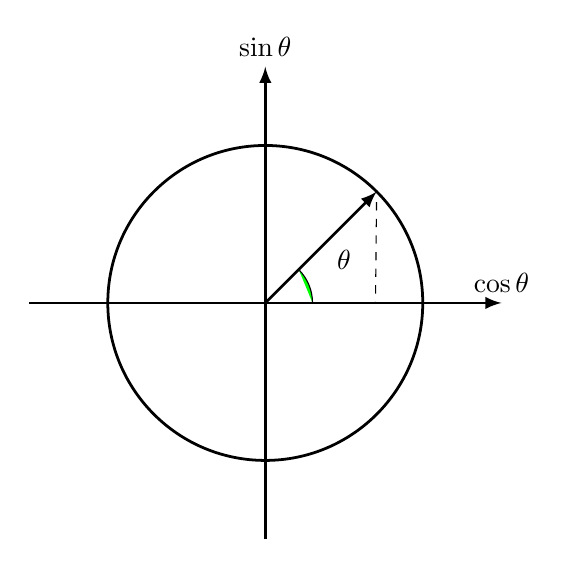
\begin{tikzpicture}
\draw[->,>=latex,line width = 1pt] (0,-3) -- (0,3) node[above] {$\sin{\theta}$};
\draw[->,>=latex,line width = 1pt] (-3,0) -- (3,0) node[above] {$\cos{\theta}$};
\node (a) at (1,.55) {$\theta$};
\draw[line width = 1pt] (0,0) circle (2cm);
\draw[->,>=latex,line width = 1pt] (0,0) -- (45:2cm) node (b) {} ;
\draw[dashed] (b) -- (1.4,0);
\draw[fill=green]
  % radius=3mm, initial=0, final=90
  %([shift={(0:3mm)}]c1) arc (0:90:3mm)
  ($(0,0) + (0:6mm)$) arc (0:45:6mm);
\end{tikzpicture}
\end{center}

$$
V(t) = V_{m} \cos{\omega t + 45^{\circ}} = V_{m} \:\: \phase{45^{\circ}}
$$



\subsubsection{نکته}

فازور برداری است که از یک فاز اولیه شروع به چرخش می کند و جهت چرخش جهت مثلثاتی است 

یک ولتاژ سینوسی با معادله ریاضی :

$$
V(t) = V_{m} \cos{\omega t + \phi}
$$

دارای فازور :

$$
V = V_{m} \phase{\phi^{\circ}}
$$

( که خوانده می شود 
$V_{m}$
با زاویه ی
$\phi$


و همچنین یک جریان الکتریکی با معادله ی 
$$
I(t) = I_{m} \cos{( \omega t + \phi )}
$$

دارای فازور 
$$
I = I_{m} \phase{\phi^{\circ}}
$$

می باشد 


باید توجه شود که برای نوشتن فازور باید فرمت حتماً کوسینوسی باشد و اگر سینوسی باشد باید ابتدا به فرم کوسینوسی تبدیل شود .

$$
\sin{\omega t} = \cos{(\omega t - \frac{\pi}{2})}
$$

$$
\cos{\omega t} = \sin{(\omega t + \frac{\pi}{2})}
$$



\section{عملیات ریاضی در حوزه ی فازور}


\subsection{ضرب}

اندازه ها در هم ضرب و زاویه ها با هم جمع می شوند 

\subsubsection{مثال}

$$
V_{1} = 4 \phase{90^{\circ}} \qquad V_{2} = 10 \phase{-45^{\circ}}
$$


\begin{align*}
V_{1} \times V_{2} &= 4 \times 10 \phase{90 + ( - 45 )} \\
&= 40 \phase{45^{\circ}} \\
&\Rightarrow V(t) = 40 \cos{\omega t + 45}
\end{align*}


\subsection{تقسیم}

اندازه ها بر هم تقسیم و زاویه ها از هم کم می شوند 


$$
V_{1} = 4 \phase{90^{\circ}} \qquad V_{2} = 10 \phase{- 45^{\circ}}
$$

\begin{align*}
V_{1} \div V_{2} &= \frac{4}{10} \phase{90 - ( - 45 )} \\
&= 40 \phase{135^{\circ}} \\
&\Rightarrow V(t) = 40 \cos{\omega t + 135}
\end{align*}



\subsection{جمع و تفریق}


در این حالت بهتر است فازور به شکل دکارتی نوشته شود 

کلاً دو نوع نمایش برای فازور داریم : 
\begin{itemize}
	\item قطبی 
	( یعنی اندازه و زاویه )
	\item دکارتی
	( یعنی حقیقی و موهومی )
\end{itemize}


\begin{itemize}
	\item در ضرب و تقسیم بهترین حالت قطبی است
	\item در جمع و تفریق بهترین حالت دکارتی است
	، در حالت دکارتی حقیقی ها با هم جمع یا تفریق می شوند و موهومی ها با هم .
\end{itemize}





\begin{center}
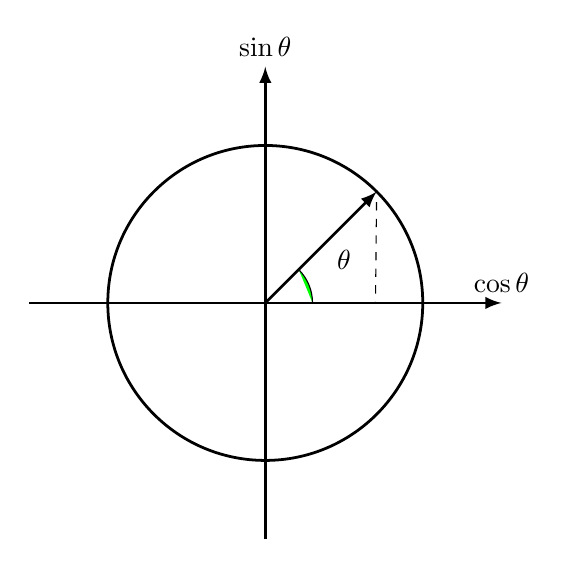
\begin{tikzpicture}
\draw[->,>=latex,line width = 1pt] (0,-3) -- (0,3) node[above] {$\sin{\theta}$};
\draw[->,>=latex,line width = 1pt] (-3,0) -- (3,0) node[above] {$\cos{\theta}$};
\node (a) at (1,.55) {$\theta$};
\draw[line width = 1pt] (0,0) circle (2cm);
\draw[->,>=latex,line width = 1pt] (0,0) -- (45:2cm) node (b) {} ;
\draw[dashed] (b) -- (1.4,0);
\draw[fill=green]
  % radius=3mm, initial=0, final=90
  %([shift={(0:3mm)}]c1) arc (0:90:3mm)
  ($(0,0) + (0:6mm)$) arc (0:45:6mm);
\end{tikzpicture}
\end{center}


$$
V = V_{m} \phase{\phi} = V_{m} \cos{\omega t + \phi}
$$


\begin{align*}
V &= ( V_{m} \cos{\phi} + V_{m} \sin{\phi} ) \\
&= V_{m} \cos{\phi} + j V_{m}\sin{\phi}
\end{align*}

$J$
یعنی 90 درجه جلوتر

\begin{center}
\begin{tikzpicture}
\node[scale = 2] (a) at (0,0) {$J$} ;
\node[scale = 2] (b) at (1.5,0) {$=$} ;
\node[scale = 2] (c) at (3,0) {جلوتر} ;
\node[scale = 2] (d) at (5,0) {$90^{\circ}$} ;
\node[scale = 2] (d) at (6.5,0) {$=$} ;
\node[scale = 2] (d) at (8.5,0) {$ 1 \phase{90^{\circ}}$} ;

\node[scale = 2] (a) at (0,-2) {$- J$} ;
\node[scale = 2] (b) at (1.5,-2) {$=$} ;
\node[scale = 2] (c) at (3,-2) {عقبتر} ;
\node[scale = 2] (d) at (5,-2) {$90^{\circ}$} ;
\node[scale = 2] (d) at (6.5,-2) {$=$} ;
\node[scale = 2] (d) at (8.5,-2) {$ 1 \phase{- 90^{\circ}}$} ;
\end{tikzpicture}
\end{center}


\subsection{تبدیل از قطبی به دکارتی}


$$
V = 4 \phase{30^{\circ}}
$$


\begin{align*}
V &= 4 \cos{30^{\circ}} + J 4 \sin{30^{\circ}} \\
&= 4 \sqrt{\frac{3}{2}} + J . 4 . \frac{1}{2} \\
&= 2 \sqrt{3} + J 2 
\end{align*}




\subsubsection{مثال}

$$
V_{1} = 4 + J 3 \qquad V_{2} = 2 - J  
$$


\begin{align*}
V_{1} + V_{2} &= 6 - 2 J \\
V_{1} - V_{2} &= 2 + 4 J \\
\end{align*}



\subsubsection{مثال}

فرض کنید جریان الکتریکی در دو شاخه ی یک مدار به صورت زیر است .

$$
I_{1}(t) = 10 \cos{(t + 30^{\circ})} \to I_{1} = 10 \phase{30^{\circ}}
$$

$$
I_{2}(t) = 5 \cos{(t + 45^{\circ})} \to I_{2} = 5 \phase{45^{\circ}}
$$


چهار عمل اصلی ریاضی را بر روی این جریان ها پیاده کنید .


\begin{align*}
I_{1} &= 10 \phase{30^{\circ}} \\
&= 10 \cos{30} + J . 10 \sin{30} \\
&= 10 \frac{\sqrt{3}}{2} + J . 10 . \frac{1}{2} \\
&= 5 \sqrt{3} + J . 5
\end{align*}



\begin{align*}
I_{2} &= 5 \phase{45^{\circ}} \\
&= 5 \cos{45} + J . 5 . \sin{45} \\
&= 5 \frac{\sqrt{2}}{2} + J . 5  \frac{\sqrt{2}}{2} \\
\end{align*}


\begin{align*}
I_{1} \times I_{2} &= 10 \times 5 \phase{30 + 45} = 50 \phase{75} \\
I_{1} / I_{2} &= 10 / 5 \phase{30 - 45} = 2 \phase{-15} \\
I_{1} + I_{2} &= ( 5 \sqrt{3} + 5 \frac{\sqrt{2}}{2} ) + J ( 5 + 5 \frac{\sqrt{2}}{2} ) \\
I_{1} - I_{2} &= ( 5 \sqrt{3} - 5 \frac{\sqrt{2}}{2} ) + J (  5 - 5 \frac{\sqrt{2}}{2} ) \\
\end{align*}




\subsubsection{نکته}

در تحلیل مدارهای سینوسی ابتدا مدار به حوزه ی فازور منتقل می شود . در حوزه ی فازور دقیقاً مثل مدارهای مقاومتی ، مدار را حل می کنیم .

پس از حل مدار و به دست آوردن مجهول نتیجه را از حوزه ی فازور به حالت  معمول بر می گردانیم .


\begin{center}
  \rowcolors{1}{codepurple}{backcolour}
  \bgroup
  \def\arraystretch{1.5}%
  \begin{tabular}{ c | c | c  }
    قطعاتی که در یک مدار داریم
     & حوزه ی غیر فازور ( زمان )
      & حوزه ی فازور
       \\ \hline
    مقاومت
     & $R$ & $R$ \\ \hline
    سلف
     & $L$ & $J.L.\omega$  \\ \hline
    خازن
     & $C$ & $\frac{1}{J.C.\omega}$  \\ \hline
    منبع ولتاژ
     & $V(t) = V_{m}\cos{(\omega t + \phi)}$ & 
     $V = V_{m} \phase{\phi}$  \\ \hline
    منبع جریان
     & $I(t) = I_{m} \cos{(\omega t + \phi)}$ & 
     $I = I_{m} \phase{\phi}$  \\ 
  \end{tabular}
  \egroup
\end{center}


\begin{tcolorbox}
$\omega$
فرکانس زاویه ای می باشد و برابر است با :
$$
\omega = 2 \pi f
$$
\end{tcolorbox}




\subsubsection{نکته}

در حوزه ی فازور سلف و خازن را همچون مقاومت در نظر می گیریم . 

سلف
 $\leftarrow$
  مقاومت القایی

خازن
  $\leftarrow$ 
  مقاومت خازنی



\subsubsection{مثال}

در مدار شکل زیر معادله ی ریاضی سلف را به دست آورید 


\begin{center}
\begin{circuitikz}[american]
\node (a) at (-2.5,0) {$V(t) = 10 \cos{(t)}$};
\node (b) at (3.5,0) {$= 1 H $};
\draw (0,-1.5) to[sI] (0,1.5);
\draw (2,1.5) to[cute choke, l=$L_{1}$] (2,-1.5);
\draw (0,1.5) to[short, f = $I$] (2,1.5);
\draw (0,-1.5) -- (2,-1.5);
\end{circuitikz}
\end{center}

مدار را به حوزه ی فازور می بریم :

\begin{center}
\begin{circuitikz}[american]
\node (a) at (-1.5,0) {$10\phase{0^{\circ}}$};
\node (b) at (5,0) {$= J.L.\omega = J \times 1 \times 1$};
\draw (0,-1.5) to[sI] (0,1.5);
\draw (2,1.5) to[cute choke, l=$L_{2}$] (2,-1.5);
\draw (0,1.5) to[short, f = $I$] (2,1.5);
\draw (0,-1.5) -- (2,-1.5);
\end{circuitikz}
\end{center}


\begin{align*}
I = \frac{V}{R} = \frac{10 \phase{0^{\circ}}}{J} = \frac{10 \phase{0^{\circ}}}{1 \phase{90^{\circ}}} = 10 \phase{-90^{\circ}}
\end{align*}

معادله ی جریان بر حسب زمان :

$$
\Rightarrow I(t) = 10 \cos{(t  - 90)}
$$




\subsubsection{مثال}

در مدار شکل زیر معادله ی ریاضی جریان خازن را به دست آورید 

\begin{center}
\begin{circuitikz}[american]
\node (a) at (-3,0) {$V(t) = 5 \cos{(2t + 45)}$};
\node (b) at (3.5,0) {$ 2 F $};
\draw (0,-1.5) to[sI] (0,1.5);
\draw (2,1.5) to[C] (2,-1.5);
\draw (0,1.5) to[short, f = $I$] (2,1.5);
\draw (0,-1.5) -- (2,-1.5);
\end{circuitikz}
\end{center}

مدار را به حوزه ی فازور می بریم :

\begin{center}
\begin{circuitikz}[american]
\node (a) at (-1.5,0) {$5\phase{45^{\circ}}$};
\node (b) at (5,0) {$ \frac{1}{J.C.\omega} = \frac{1}{J \times 2 \times 2} = \frac{1}{4 J} $};
\draw (0,-1.5) to[sI] (0,1.5);
\draw (2,1.5) to[C] (2,-1.5);
\draw (0,1.5) to[short, f = $I$] (2,1.5);
\draw (0,-1.5) -- (2,-1.5);
\end{circuitikz}
\end{center}



\begin{align*}
I = \frac{V}{R} = \frac{ 5 \phase{45} }{ \cfrac{1}{4J} } = 5 \phase{45} \times 4 \phase{90} = 20 \phase{135}
\end{align*}


معادله ی جریان بر حسب زمان :


$$
\Rightarrow I(t) = 20 \cos{(2t + 135)}
$$



\subsubsection{نکته}

\begin{tcolorbox}
{
\Large
$$
\frac{1}{J} = - J
$$
}
\end{tcolorbox}


\subsubsection{مثال}


در مدار شکل زیر معادله ی ریاضی جریان را به دست آورید 

\begin{center}
\begin{circuitikz}[american]
\node (a) at (-2.5,0) {$V(t) = 5 \cos{(t)}$};
\node (b) at (3.5,0.75) {$ 2 F $};
\node (c) at (3.5,-0.75) {$ \frac{1}{2} F $};
\draw (0,-1.5) to[sI] (0,1.5);
\draw (2,1.5)  to[cute choke]  (2,0)  to[C] (2,-1.5);
\draw (0,1.5) to[short, f = $I$] (2,1.5);
\draw (0,-1.5) -- (2,-1.5);
\end{circuitikz}
\end{center}

مدار را به حوزه ی فازور می بریم :

\begin{center}
\begin{circuitikz}[american]
\node (a) at (-1.5,0) {$ 5 \phase{0} $};
\node (b) at (4.5,0.75) {$ J . C . \omega = J \times 1 \times 1 = J $};
\node (c) at (5.5,-0.75) {$ \frac{1}{J . C . \omega} = \frac{1}{ J \times \frac{1}{2} \times 1 }  = \frac{1}{\frac{1}{2} J} = \frac{2}{J} = - 2 J $};
\draw (0,-1.5) to[sI] (0,1.5);
\draw (2,1.5)  to[cute choke]  (2,0)  to[C] (2,-1.5);
\draw (0,1.5) to[short, f = $I$] (2,1.5);
\draw (0,-1.5) -- (2,-1.5);
\end{circuitikz}
\end{center}

مقاومت معادل :

$$
R_{T} = J + ( - 2 J ) = - J  
$$



\begin{align*}
I = \frac{V}{R} = \frac{5 \phase{0} }{- J} = \frac{5 \phase{0}}{1 \phase{-90}} = 5 \phase{0 - (-90)} = 5 \phase{90}
\end{align*}

معادله ی جریان بر حسب زمان :


$$
I(t) = 5 \cos{(t + 90)}
$$



\subsubsection{نکته}


منظور از مدار در مثال ها یک مدار الکتریکی در حالت دائمی سینوسی می باشد 

\subsubsection{مثال}

در مدار شکل زیر جریان سلف و جریان خازن را رسم کرده و دیگرام برداری را برای ولتاژها و جریان ها رسم کنید .


\begin{center}
\begin{circuitikz}[american]
\node (a) at (-2,0) {$ I = 10 \cos{(t)} $};
\node (b) at (7,0) {$ 2 H $};
\draw (0,-1.5) to[sI] (0,1.5);
\draw (0,1.5) -- (6,1.5);
\draw (3,1.5) to[C=1<\farad>] (3,-1.5);
\draw (6,-1.5) -- (0,-1.5);
\draw (6,-1.5) to[cute choke] (6,1.5);
\end{circuitikz}
\end{center}

مدار را به حوزه ی فازور می بریم :

\begin{center}
\begin{circuitikz}[american]
\node (a) at (-2,0) {$ I = 10 \phase{0} $};
\node (b) at (7,0) {$ J . L . \omega $};
\node (c) at (4,0) {$ \frac{1}{J . C . \omega} $};
\draw (0,-1.5) to[sI] (0,1.5);
\draw (0,1.5) -- (6,1.5);
\draw (3,1.5) to[C] (3,-1.5);
\draw (6,-1.5) -- (0,-1.5);
\draw (6,-1.5) to[cute choke] (6,1.5);
\end{circuitikz}
\end{center}

$$
J . L . \omega = J \times 2 \times 1 = 2 J
$$

$$
\frac{1}{J . C . \omega} = \frac{1}{ J \times 1 \times 1} = \frac{1}{J} = - J
$$



\begin{align*}
I_{C} = \frac{2J}{-J + 2J} \times 10 \phase{0} = \frac{2J}{J} \times 10 \phase{0} = 2 \times 10 \phase{0} = 20 \phase{0}
\end{align*}


\begin{align*}
\frac{2J}{J} = \frac{2 \phase{90}}{1 \phase{90}} = 2 \phase{90 - 90} = 2 \phase{0} = 2
\end{align*}





\begin{align*}
I_{L} = \frac{-J}{-J + 2J} \times 10 \phase{0} = \frac{-J}{+J} \times 10 \phase{0} = -10 \phase{0} = 10 \phase{180}
\end{align*}



\begin{align*}
\frac{1\phase{-90}}{1\phase{90}} = 1 \phase{-180} = 1 \phase{180}
\end{align*}


\begin{align*}
I_{C}(t) &= 20 \cos{(20t)} \\
I_{L}(t) &= 10 \cos{(t + 180)} = 10 \cos{(t - 180)}
\end{align*}



\begin{align*}
V_{C} = R_{C} I_{C} = -J \times 20 \phase{0} = 1 \phase{-90} \times 20 \phase{0} = 20 \phase{-90} = -20J
\end{align*}




\begin{align*}
V_{L} = R_{L} I_{L} = 2J \times 10 \phase{180} = 2 \phase{90} \times 10 \phase{180} = 20 \phase{270} = 20 \phase{-90} = -20 J
\end{align*}





\begin{center}
\begin{tikzpicture}
\draw[dashed,->,>=latex,line width = 1pt] (0,-3) -- (0,3) node[above] {$\sin{\theta}$};
\draw[dashed,->,>=latex,line width = 1pt] (-3,0) -- (3,0) node[right] {$\cos{\theta}$};
\draw[->,>=latex,line width = 1pt] (.1,0.2) -- (2,0.2) node[above right] {$I_{C}(t) = 20 \cos{(t)} = 20 \phase{0}$};
\draw[->,>=latex,line width = 1pt] (-.1,0.2) -- (-1,0.2) node[above left] {$I_{L}(t) = 10 \cos{(t + 180)} = 10 \phase{180}$};
%\draw (-.1,0.4) -- (2,0.4) node[above] {$$};
\draw[->,>=latex,line width = 1pt] (-0.1,-0.1) -- (-0.1,-1) node[below] {$V_{L}(t) = V_{C}(t)$};
%\draw[->,>=latex,line width = 1pt] (0,0) -- (45:2cm) node (b) {} ;
%\draw[dashed] (b) -- (1.4,0);
\end{tikzpicture}
\end{center}



\begin{tcolorbox}
\begin{itemize}
	\item جریان خازن 90 درجه نسبت به ولتاژش جلوتر
	(پیش فاز) است
	\item جریان سلف 90 درجه نسبت به ولتاژش
	(پس فاز) است
	\item جریان و ولتاژ مقاومت
	هم فاز هستند
\end{itemize}

اثبات :

\begin{align*}
I_{C} = \frac{V_{C}}{X_{C}} = \frac{V_{C}}{\frac{1}{J.C.\omega}} = (V_{C} . C . \omega) J = (V_{C} . C . \omega) \times 1 \phase{90^{\circ}}
\end{align*}



\begin{align*}
I_{L} = \frac{V_{L}}{X_{L}} = \frac{V_{L}}{J . L . \omega} = \left( \frac{V_{L}}{L . \omega} \right) \times \frac{1}{J} = \left( \frac{V_{L}}{L . \omega} \right) \times - J  = \left( \frac{V_{L}}{L . \omega} \right) \times 1 \phase{-90^{\circ}}
\end{align*}



\begin{align*}
I_{R} = \frac{V_{R}}{R}
\end{align*}

\end{tcolorbox}


\newpage

\subsubsection{مثال}


در مدار شکل زیر ولتاژ دو سر مقاومت و ولتاژ دو سر سلف را به دست آورده و دیاگرام برداری مربوط به آن را رسم کنید 

\begin{center}
\begin{circuitikz}[american]
\node (a) at (-2,0) {$ I = 10 \cos{(2t)} $};
\node (b) at (4.5,2) {$ 2 H $};
\draw (0,-1.5) to[V] (0,1.5);
\draw (0,1.5) to[R=$4 \:\: \Omega$] (3,1.5) to[cute choke] (6,1.5);
\draw (6,-1.5) -- (0,-1.5);
\draw (6,-1.5) -- (6,1.5);
\end{circuitikz}
\end{center}

مدار را به حوزه ی فازور می بریم :

\begin{center}
\begin{circuitikz}[american]
\node (a) at (-2,0) {$ I = 10\phase{0} $};
\node (b) at (4.5,2.2) {$J . L . \omega = 4 J$};
\draw (0,-1.5) to[V] (0,1.5);
\draw (0,1.5) to[R=$4 \:\: \Omega$] (3,1.5) to[cute choke] (6,1.5);
\draw (6,-1.5) -- (0,-1.5);
\draw (6,-1.5) -- (6,1.5);
\end{circuitikz}
\end{center}

\begin{align*}
Z = R_{T} = 4 + 4 J
\end{align*}





\begin{align*}
\tan{\theta} &= \frac{4}{4} = 1 \Rightarrow \theta = \frac{\pi}{4} = 45^{\circ} \\
r &= \sqrt{4^{2} + 4^{2}} = \sqrt{2 \times 16} = 4 \sqrt{2} \\
&\Rightarrow R_{T} = 4\sqrt{2} \phase{45^{\circ}}
\end{align*}





\begin{align*}
I = \frac{V}{R} = \frac{10 \phase{0} }{ 4 \sqrt{2} \phase{45} } = \frac{10}{4\sqrt{2} } \phase{-45} \\
\end{align*}




\begin{align*}
V_{R} = R \times I = 4 \times \frac{10}{4\sqrt{2}} \phase{-45} = \frac{10}{\sqrt{2}} \phase{-45} 
\end{align*}

$$
\Rightarrow V_{R}(t) = \frac{10}{\sqrt{2}} \cos{(2t - 45)}
$$



\begin{align*}
V_{L}(t) = R_{L} \times I = 4 J \times \frac{10}{4 \sqrt{2} } \phase{-45} = 4 \phase{90} \times \frac{10}{4\sqrt{2}} \phase{-45} = \frac{10}{\sqrt{2}} \phase{45}
\end{align*}

$$
\Rightarrow V_{L} = \frac{10}{\sqrt{2}} \cos{(2t + 45)}
$$






\begin{center}
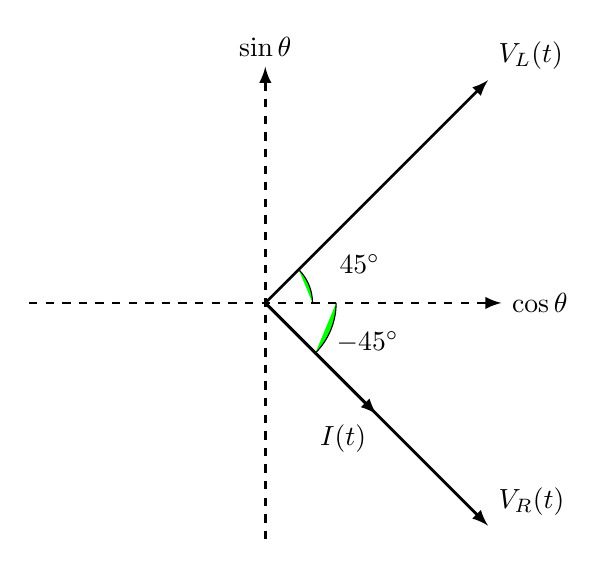
\begin{tikzpicture}
\draw[dashed,->,>=latex,line width = 1pt] (0,-3) -- (0,3) node[above] {$\sin{\theta}$};
\draw[dashed,->,>=latex,line width = 1pt] (-3,0) -- (3,0) node[right] {$\cos{\theta}$};
\node (a) at (1.2,.5) {$45^{\circ}$};
\node (aa) at (1.3,-.5) {$-45^{\circ}$};
\draw[->,>=latex,line width = 1pt] (0,0) -- (45:4cm) node[above right ] (b) {$V_{L}(t)$} ;
\draw[->,>=latex,line width = 1pt] (0,0) -- (-45:4cm) node[above right ] (c) {$V_{R}(t)$} ;
\draw[->,>=latex,line width = 1pt] (0,0) -- (-45:2cm) node[below left ] (d) {$I(t)$} ;
\draw[fill=green]
  % radius=3mm, initial=0, final=90
  %([shift={(0:3mm)}]c1) arc (0:90:3mm)
  ($(0,0) + (0:6mm)$) arc (0:45:6mm);
\draw[fill=green]
  % radius=3mm, initial=0, final=90
  %([shift={(0:3mm)}]c1) arc (0:90:3mm)
  ($(0,0) + (0:9mm)$) arc (0:-45:9mm);
\end{tikzpicture}
\end{center}



\section{تشدید ( رزونانس )}


جریان خیلی شدید به خاطر اتصال کوتاه در مدار اتفاق می افتد .\\
\\ 


\begin{center}
\begin{circuitikz}[american]
\node (a) at (1.5,2.2) {$- J$};
\node (b) at (4.5,2.2) {$J$};
\draw (0,-1.5) to[V] (0,1.5);
\draw (0,1.5) to[C] (3,1.5) to[cute choke] (6,1.5);
\draw (6,-1.5) -- (0,-1.5);
\draw (6,-1.5) -- (6,1.5);
\end{circuitikz}
\end{center}

.\\

\begin{center}
\begin{circuitikz}[american]
\node (a) at (-.8,1) {$- J$};
\node (b) at (-.8,-1) {$J$};
\draw (0,2) to[C] (0,0) to[cute choke] (0,-2);
\begin{scope}[xshift=3cm]
\node (a) at (0,0) {$\Rightarrow$};
\end{scope}
\begin{scope}[xshift=6cm]
\draw (0,1) -- (0,-1);
\draw (0,2) to[short, -*] (0,1);
\draw (0,-2) to[short, -*] (0,-1);
\end{scope}
\end{circuitikz}
\end{center}


$$
R_{T} = - J + J = 0
$$


\begin{center}
\begin{circuitikz}[american]
\node (a) at (-1.8,0) {$- J$};
\node (b) at (1.8,0) {$J$};
\draw (-1,1) to[C] (-1,-1);
\draw (1,1) to[cute choke] (1,-1);
\draw (-1,1) -- (1,1);
\draw (-1,-1) -- (1,-1);
\draw (0,2) -- (0,1);
\draw (0,-1) -- (0,-2);
\begin{scope}[xshift=3cm]
\node (a) at (0,0) {$\Rightarrow$};
\end{scope}
\begin{scope}[xshift=6cm]
\draw (0,2) to[short, -*] (0,1);
\draw (0,-2) to[short, -*] (0,-1);
\end{scope}
\end{circuitikz}
\end{center}

$$
R_{T} = \frac{- J \times J}{- J + J} = \frac{1 \phase{-90} \times 1 \phase{90}}{0} = \frac{1 \phase{0}}{0} = \frac{1}{0}
$$


\end{document}